\documentclass[a4paper]{article}

\newcommand{\triposcourse}{Markov Chains}
\usepackage{fancyhdr,titlesec,geometry}
\usepackage[dvipsnames]{xcolor}
\usepackage[many]{tcolorbox}
\usepackage{xifthen}
\usepackage{import}
\usepackage{parskip}
\usepackage{transparent}
\usepackage{mathtools,amssymb,amsfonts,amsthm,bm}   % Math Presets
\usepackage{array,tabularx,booktabs}                % Table Presets
\usepackage{graphicx,wrapfig,float,caption}         % Figure Presets
\usepackage{setspace,multicol}                      % Text Presets
\usepackage{tikz,physics,cancel,tkz-euclide,pgfplots,tikz-3dplot}                    % Physics Presets
\usepackage{amsmath}
\usepackage{mathrsfs}
\usepackage{enumerate}
\usepackage[shortlabels]{enumitem}
\usepackage{hyperref}
\usepackage{lipsum}
\usepackage{IEEEtrantools}
\usepackage{xcomment}
\usepackage{sectsty}
\usepackage{thmtools}
\usepackage{mdframed}
\usepackage{siunitx}
\usepackage{centernot}

\newcommand{\sectionbreak}{\clearpage}

\tdplotsetmaincoords{60}{120}

\usetikzlibrary{arrows.meta}
\usetikzlibrary{decorations.markings}
\usetikzlibrary{decorations.pathmorphing}
\usetikzlibrary{automata, positioning}
\usetikzlibrary{fadings}
\usetikzlibrary{intersections}
\usetikzlibrary{cd}
\usetikzlibrary{patterns}
\usetikzlibrary{shapes.arrows}
\usepgfplotslibrary{colormaps, external}
\pgfarrowsdeclarecombine{twolatex'}{twolatex'}{latex'}{latex'}{latex'}{latex'}
\tikzset{->/.style = {decoration={markings,
                                  mark=at position 1 with {\arrow[scale=1.6]{latex'}}},
                      postaction={decorate}}}
\tikzset{<-/.style = {decoration={markings,
                                  mark=at position 0 with {\arrowreversed[scale=1.6]{latex'}}},
                      postaction={decorate}}}
\tikzset{<->/.style = {decoration={markings,
                                   mark=at position 0 with {\arrowreversed[scale=1.6]{latex'}},
                                   mark=at position 1 with {\arrow[scale=1.6]{latex'}}},
                       postaction={decorate}}}
\tikzset{->-/.style = {decoration={markings,
                                   mark=at position #1 with {\arrow[scale=1.6]{latex'}}},
                       postaction={decorate}}}
\tikzset{-<-/.style = {decoration={markings,
                                   mark=at position #1 with {\arrowreversed[scale=1.6]{latex'}}},
                       postaction={decorate}}}
\tikzset{->>/.style = {decoration={markings,
                                  mark=at position 1 with {\arrow[scale=1.6]{twolatex'}}},
                      postaction={decorate}}}
\tikzset{<<-/.style = {decoration={markings,
                                  mark=at position 0 with {\arrowreversed[scale=1.6]{twolatex'}}},
                      postaction={decorate}}}
\tikzset{<<->>/.style = {decoration={markings,
                                   mark=at position 0 with {\arrowreversed[scale=1.6]{twolatex'}},
                                   mark=at position 1 with {\arrow[scale=1.6]{twolatex'}}},
                       postaction={decorate}}}
\tikzset{->>-/.style = {decoration={markings,
                                   mark=at position #1 with {\arrow[scale=1.6]{twolatex'}}},
                       postaction={decorate}}}
\tikzset{-<<-/.style = {decoration={markings,
                                   mark=at position #1 with {\arrowreversed[scale=1.6]{twolatex'}}},
                       postaction={decorate}}}

\tikzset{
set arrow inside/.code={\pgfqkeys{/tikz/arrow inside}{#1}},
set arrow inside={end/.initial=>, opt/.initial=},
/pgf/decoration/Mark/.style={
    mark/.expanded=at position #1 with
    {
        \noexpand\arrow[\pgfkeysvalueof{/tikz/arrow inside/opt}]{\pgfkeysvalueof{/tikz/arrow inside/end}}
    }
},
arrow inside/.style 2 args={
    set arrow inside={#1},
    postaction={
        decorate,decoration={
            markings,Mark/.list={#2}
        }
    }
},
}

\tikzstyle{circ}=[fill=black, draw=black, shape=circle]
\tikzset{
dot/.style = {circle, fill, minimum size=#1,
              inner sep=0pt, outer sep=0pt},
dot/.default = 5pt% size of the circle diameter 
}
\tikzset{mstate/.style={circle, draw, blue, text=black, minimum width=0.7cm}}
\tikzset{snake it/.style={-stealth,
decoration={snake, 
    amplitude = .4mm,
    segment length = 2mm,
    post length=0.9mm},decorate}}

\def\centerarc[#1](#2)(#3:#4:#5)% Syntax: [draw options](center)(initial angle:final angle:radius)
    { \draw[#1] ($(#2)+({#5*cos(#3)},{#5*sin(#3)})$) arc (#3:#4:#5); }

\hypersetup{
    colorlinks=true,
    linkcolor=blue,
    filecolor=blue,
    citecolor = black,      
    urlcolor=cyan,
    }

%%%%%%%%%%% Snippets %%%%%%%%%%%%%%%%
\newcommand*\widefbox[1]{\fbox{\hspace{2em}#1\hspace{2em}}}
\newcommand{\xint}{\int_{x_1}^{x_2}}
\newcommand{\mw}{\sqrt{m\omega}}
\newcommand{\de}{\delta}
\newcommand{\dde}{\dot{\delta}}
\newcommand{\di}{\delta_i}
\newcommand{\ddi}{\dot{\delta_i}}
\newcommand{\dddi}{\ddot{\delta_i}}
\newcommand{\dipl}{\delta_{i+1}}
\newcommand{\dimi}{\delta_{i-1}}
\newcommand{\ddt}[1]{\frac{{d} #1}{dt}}
\newcommand{\ddtt}[1]{\frac{d^2 #1}{dt^2}}
\newcommand{\ddx}[1]{\frac{d #1}{dx}}
\newcommand{\ddxx}[1]{\frac{d^2 #1}{dx^2}}
\newcommand{\eps}{\epsilon}
\newcommand{\del}[2]{\frac{\partial #1}{\partial #2}}
\newcommand{\deltwo}[2]{\frac{\partial^2 #1}{\partial #2^2}}
\newcommand{\lam}{\lambda}
\newcommand{\Lam}{\Lambda}
\newcommand{\sig}{\sigma}
\newcommand{\Sig}{\Sigma}
\newcommand{\half}{\frac{1}{2}}
\newcommand{\munu}{{\mu\nu}}
\newcommand{\thalf}{\tfrac{1}{2}}
\renewcommand{\div}{\nabla\cdot}
\renewcommand{\curl}{\nabla\times}

\DeclareMathOperator{\orb}{Orb}
\DeclareMathOperator{\stab}{Stab}
\DeclareMathOperator{\adj}{adj}
\DeclareMathOperator{\ccl}{ccl}
\let\var\relax
\DeclareMathOperator{\var}{Var}
\DeclareMathOperator{\cov}{Cov}
\DeclareMathOperator{\corr}{Corr}
\DeclareMathOperator{\Markov}{Markov}
\DeclareMathOperator{\nullity}{nullity}

\newcommand{\bfA}{{\bf A}}
\newcommand{\bfB}{{\bf B}}
\newcommand{\bfC}{{\bf C}}
\newcommand{\bfD}{{\bf D}}
\newcommand{\bfE}{{\bf E}}
\newcommand{\bfF}{{\bf F}}
\newcommand{\bfG}{{\bf G}}
\newcommand{\bfH}{{\bf H}}
\newcommand{\bfI}{{\bf I}}
\newcommand{\bfJ}{{\bf J}}
\newcommand{\bfK}{{\bf K}}
\newcommand{\bfL}{{\bf L}}
\newcommand{\bfM}{{\bf M}}
\newcommand{\bfN}{{\bf N}}
\newcommand{\bfO}{{\bf O}}
\newcommand{\bfP}{{\bf P}}
\newcommand{\bfQ}{{\bf Q}}
\newcommand{\bfR}{{\bf R}}
\newcommand{\bfS}{{\bf S}}
\newcommand{\bfT}{{\bf T}}
\newcommand{\bfU}{{\bf U}}
\newcommand{\bfV}{{\bf V}}
\newcommand{\bfW}{{\bf W}}
\newcommand{\bfX}{{\bf X}}
\newcommand{\bfY}{{\bf Y}}
\newcommand{\bfZ}{{\bf Z}}

\newcommand{\bfa}{{\bf a}}
\newcommand{\bfb}{{\bf b}}
\newcommand{\bfc}{{\bf c}}
\newcommand{\bfd}{{\bf d}}
\newcommand{\bfe}{{\bf e}}
\newcommand{\bff}{{\bf f}}
\newcommand{\bfg}{{\bf g}}
\newcommand{\bfh}{{\bf h}}
\newcommand{\bfi}{{\bf i}}
\newcommand{\bfj}{{\bf j}}
\newcommand{\bfk}{{\bf k}}
\newcommand{\bfl}{{\bf l}}
\newcommand{\bfm}{{\bf m}}
\newcommand{\bfn}{{\bf n}}
\newcommand{\bfo}{{\bf o}}
\newcommand{\bfp}{{\bf p}}
\newcommand{\bfq}{{\bf q}}
\newcommand{\bfr}{{\bf r}}
\newcommand{\bfs}{{\bf s}}
\newcommand{\bft}{{\bf t}}
\newcommand{\bfu}{{\bf u}}
\newcommand{\bfv}{{\bf v}}
\newcommand{\bfw}{{\bf w}}
\newcommand{\bfx}{{\bf x}}
\newcommand{\bfy}{{\bf y}}
\newcommand{\bfz}{{\bf z}}

\newcommand{\mcA}{{\mathcal{A}}}
\newcommand{\mcB}{{\mathcal{B}}}
\newcommand{\mcC}{{\mathcal{C}}}
\newcommand{\mcD}{{\mathcal{D}}}
\newcommand{\mcE}{{\mathcal{E}}}
\newcommand{\mcF}{{\mathcal{F}}}
\newcommand{\mcG}{{\mathcal{G}}}
\newcommand{\mcH}{{\mathcal{H}}}
\newcommand{\mcI}{{\mathcal{I}}}
\newcommand{\mcJ}{{\mathcal{J}}}
\newcommand{\mcK}{{\mathcal{K}}}
\newcommand{\mcL}{{\mathcal{L}}}
\newcommand{\mcM}{{\mathcal{M}}}
\newcommand{\mcN}{{\mathcal{N}}}
\newcommand{\mcO}{{\mathcal{O}}}
\newcommand{\mcP}{{\mathcal{P}}}
\newcommand{\mcQ}{{\mathcal{Q}}}
\newcommand{\mcR}{{\mathcal{R}}}
\newcommand{\mcS}{{\mathcal{S}}}
\newcommand{\mcT}{{\mathcal{T}}}
\newcommand{\mcU}{{\mathcal{U}}}
\newcommand{\mcV}{{\mathcal{V}}}
\newcommand{\mcW}{{\mathcal{W}}}
\newcommand{\mcX}{{\mathcal{X}}}
\newcommand{\mcY}{{\mathcal{Y}}}
\newcommand{\mcZ}{{\mathcal{Z}}}

\newcommand{\bbA}{{\mathbb{A}}}
\newcommand{\bbB}{{\mathbb{B}}}
\newcommand{\bbC}{{\mathbb{C}}}
\newcommand{\bbD}{{\mathbb{D}}}
\newcommand{\bbE}{{\mathbb{E}}}
\newcommand{\bbF}{{\mathbb{F}}}
\newcommand{\bbG}{{\mathbb{G}}}
\newcommand{\bbH}{{\mathbb{H}}}
\newcommand{\bbI}{{\mathbb{I}}}
\newcommand{\bbJ}{{\mathbb{J}}}
\newcommand{\bbK}{{\mathbb{K}}}
\newcommand{\bbL}{{\mathbb{L}}}
\newcommand{\bbM}{{\mathbb{M}}}
\newcommand{\bbN}{{\mathbb{N}}}
\newcommand{\bbO}{{\mathbb{O}}}
\newcommand{\bbP}{{\mathbb{P}}}
\newcommand{\bbQ}{{\mathbb{Q}}}
\newcommand{\bbR}{{\mathbb{R}}}
\newcommand{\bbS}{{\mathbb{S}}}
\newcommand{\bbT}{{\mathbb{T}}}
\newcommand{\bbU}{{\mathbb{U}}}
\newcommand{\bbV}{{\mathbb{V}}}
\newcommand{\bbW}{{\mathbb{W}}}
\newcommand{\bbX}{{\mathbb{X}}}
\newcommand{\bbY}{{\mathbb{Y}}}
\newcommand{\bbZ}{{\mathbb{Z}}}

\newcommand{\mfa}{{\mathfrak{a}}}
\newcommand{\mfb}{{\mathfrak{b}}}
\newcommand{\mfc}{{\mathfrak{c}}}
\newcommand{\mfd}{{\mathfrak{d}}}
\newcommand{\mfe}{{\mathfrak{e}}}
\newcommand{\mff}{{\mathfrak{f}}}
\newcommand{\mfg}{{\mathfrak{g}}}
\newcommand{\mfh}{{\mathfrak{h}}}
\newcommand{\mfi}{{\mathfrak{i}}}
\newcommand{\mfj}{{\mathfrak{j}}}
\newcommand{\mfk}{{\mathfrak{k}}}
\newcommand{\mfl}{{\mathfrak{l}}}
\newcommand{\mfm}{{\mathfrak{m}}}
\newcommand{\mfn}{{\mathfrak{n}}}
\newcommand{\mfo}{{\mathfrak{o}}}
\newcommand{\mfp}{{\mathfrak{p}}}
\newcommand{\mfq}{{\mathfrak{q}}}
\newcommand{\mfr}{{\mathfrak{r}}}
\newcommand{\mfs}{{\mathfrak{s}}}
\newcommand{\mft}{{\mathfrak{t}}}
\newcommand{\mfu}{{\mathfrak{u}}}
\newcommand{\mfv}{{\mathfrak{v}}}
\newcommand{\mfw}{{\mathfrak{w}}}
\newcommand{\mfx}{{\mathfrak{x}}}
\newcommand{\mfy}{{\mathfrak{y}}}
\newcommand{\mfz}{{\mathfrak{z}}}

\newcommand{\mfA}{{\mathfrak{A}}}
\newcommand{\mfB}{{\mathfrak{B}}}
\newcommand{\mfC}{{\mathfrak{C}}}
\newcommand{\mfD}{{\mathfrak{D}}}
\newcommand{\mfE}{{\mathfrak{E}}}
\newcommand{\mfF}{{\mathfrak{F}}}
\newcommand{\mfG}{{\mathfrak{G}}}
\newcommand{\mfH}{{\mathfrak{H}}}
\newcommand{\mfI}{{\mathfrak{I}}}
\newcommand{\mfJ}{{\mathfrak{J}}}
\newcommand{\mfK}{{\mathfrak{K}}}
\newcommand{\mfL}{{\mathfrak{L}}}
\newcommand{\mfM}{{\mathfrak{M}}}
\newcommand{\mfN}{{\mathfrak{N}}}
\newcommand{\mfO}{{\mathfrak{O}}}
\newcommand{\mfP}{{\mathfrak{P}}}
\newcommand{\mfQ}{{\mathfrak{Q}}}
\newcommand{\mfR}{{\mathfrak{R}}}
\newcommand{\mfS}{{\mathfrak{S}}}
\newcommand{\mfT}{{\mathfrak{T}}}
\newcommand{\mfU}{{\mathfrak{U}}}
\newcommand{\mfV}{{\mathfrak{V}}}
\newcommand{\mfW}{{\mathfrak{W}}}
\newcommand{\mfX}{{\mathfrak{X}}}
\newcommand{\mfY}{{\mathfrak{Y}}}
\newcommand{\mfZ}{{\mathfrak{Z}}}

\newcommand{\rma}{\mathrm{a}}
\newcommand{\rmb}{\mathrm{b}}
\newcommand{\rmc}{\mathrm{c}}
\newcommand{\rmd}{\mathrm{d}}
\renewcommand{\dd}{\,\mathrm{d}}
\newcommand{\rme}{\mathrm{e}}
\newcommand{\rmf}{\mathrm{f}}
\newcommand{\rmg}{\mathrm{g}}
\newcommand{\rmh}{\mathrm{h}}
\newcommand{\rmi}{\mathrm{i}}
\newcommand{\rmj}{\mathrm{j}}
\newcommand{\rmk}{\mathrm{k}}
\newcommand{\rml}{\mathrm{l}}
\newcommand{\rmm}{\mathrm{m}}
\newcommand{\rmn}{\mathrm{n}}
\newcommand{\rmo}{\mathrm{o}}
\newcommand{\rmp}{\mathrm{p}}
\newcommand{\rmq}{\mathrm{q}}
\newcommand{\rmr}{\mathrm{r}}
\newcommand{\rms}{\mathrm{s}}
\newcommand{\rmt}{\mathrm{t}}
\newcommand{\rmu}{\mathrm{u}}
\newcommand{\rmv}{\mathrm{v}}
\newcommand{\rmw}{\mathrm{w}}
\newcommand{\rmx}{\mathrm{x}}
\newcommand{\rmy}{\mathrm{y}}
\newcommand{\rmz}{\mathrm{z}}
\newcommand{\rmA}{\mathrm{A}}
\newcommand{\rmB}{\mathrm{B}}
\newcommand{\rmC}{\mathrm{C}}
\newcommand{\rmD}{\mathrm{D}}
\newcommand{\rmE}{\mathrm{E}}
\newcommand{\rmF}{\mathrm{F}}
\newcommand{\rmG}{\mathrm{G}}
\newcommand{\rmH}{\mathrm{H}}
\newcommand{\rmI}{\mathrm{I}}
\newcommand{\rmJ}{\mathrm{J}}
\newcommand{\rmK}{\mathrm{K}}
\newcommand{\rmL}{\mathrm{L}}
\newcommand{\rmM}{\mathrm{M}}
\newcommand{\rmN}{\mathrm{N}}
\newcommand{\rmO}{\mathrm{O}}
\newcommand{\rmP}{\mathrm{P}}
\newcommand{\rmQ}{\mathrm{Q}}
\newcommand{\rmR}{\mathrm{R}}
\newcommand{\rmS}{\mathrm{S}}
\newcommand{\rmT}{\mathrm{T}}
\newcommand{\rmU}{\mathrm{U}}
\newcommand{\rmV}{\mathrm{V}}
\newcommand{\rmW}{\mathrm{W}}
\newcommand{\rmX}{\mathrm{X}}
\newcommand{\rmY}{\mathrm{Y}}
\newcommand{\rmZ}{\mathrm{Z}}

\newcommand{\GL}{\mathrm{GL}}
\newcommand{\Or}{\mathrm{O}}
\newcommand{\PGL}{\mathrm{PGL}}
\newcommand{\PSL}{\mathrm{PSL}}
\newcommand{\PSO}{\mathrm{PSO}}
\newcommand{\PSU}{\mathrm{PSU}}
\newcommand{\SL}{\mathrm{SL}}
\newcommand{\SO}{\mathrm{SO}}
\newcommand{\Spin}{\mathrm{Spin}}
\newcommand{\Sp}{\mathrm{Sp}}
\newcommand{\SU}{\mathrm{SU}}
\newcommand{\Mat}{\mathrm{Mat}}

% Some common notations

\renewcommand{\v}{\mathbf{v}}
\newcommand{\w}{\mathbf{w}}
\renewcommand{\u}{\mathbf{u}}

% Matrix algebras
\newcommand{\gl}{\mathfrak{gl}}
\newcommand{\ort}{\mathfrak{o}}
\newcommand{\so}{\mathfrak{so}}
\newcommand{\su}{\mathfrak{su}}
\newcommand{\uu}{\mathfrak{u}}
\renewcommand{\sl}{\mathfrak{sl}}
\newcommand{\inner}[1]{\left\langle{#1}\right\rangle}
\DeclareMathOperator{\spn}{span}

\newcommand{\mobius}{{M\"{o}bius }}

\renewcommand{\ge}{\geqslant}
\renewcommand{\le}{\leqslant}
\renewcommand{\geq}{\geqslant}
\renewcommand{\leq}{\leqslant}
\renewcommand{\restriction}{\mathord{\upharpoonright}}

\newcommand\independent{\protect\mathpalette{\protect\independenT}{\perp}}
\def\independenT#1#2{\mathrel{\rlap{$#1#2$}\mkern2mu{#1#2}}}

\setlength{\parindent}{0pt}
% \setlength{\parskip}{\baselineskip}
\newcommand{\incfig}[1]{%
    \def\svgwidth{0.4\columnwidth}
    \import{./figures/}{#1.pdf_tex}
}
%%%%%%%%%%%%%%%%%%%%%%%%%%%%%%%%%%%%%

\usepackage[T1]{fontenc}
\usepackage{lmodern,mathrsfs}

%%%%%%%boxed enviroment for final layout%%%%%%%%%%%%%

\newtheoremstyle{mystyle}%
  {}%
  {}%
  {}%
  {}%
  {\sffamily\bfseries}%
  {.}%
  { }%
  {}%

% \renewenvironment{proof}{{\sffamily\bfseries Proof. }}{\qed}

\theoremstyle{mystyle}{
  \newtheorem{theorem}{Theorem}[section]
  \newtheorem{lemma}[theorem]{Lemma}
  \newtheorem{proposition}[theorem]{Proposition}
  \newtheorem{corollary}[theorem]{Corollary}
  \newtheorem{problem}[theorem]{Problem}
  \newtheorem*{claim}{Claim}
  \newtheorem*{slemma}{Lemma}
  \newtheorem*{sprop}{Proposition}
  \newtheorem*{notation}{Notation}

  \newtheorem{inquestion}{Question}
  \newtheorem*{sque}{Question}

  \newtheorem{definition}{Definition}[section]
  \newtheorem{conjecture}{Conjecture}[section]
  \newtheorem{example}{Example}[section]
  \newtheorem*{law}{Law}

  \newtheorem*{remark}{Remark}
  \newtheorem*{note}{Note}
}

\newenvironment{question}[1]
{\renewcommand\theinquestion{#1}\inquestion}
{\endinquestion}

\theoremstyle{definition}{
    \newtheorem*{exercise}{Exercise}}

\tcolorboxenvironment{definition}{
  boxrule=0pt,
  boxsep=2pt,
  colback={White!90!Cerulean},
  enhanced jigsaw, 
  borderline west={2pt}{0pt}{Cerulean},
  sharp corners,
  before skip=10pt,
  after skip=10pt,
  breakable,
  % parbox=false,
}

\tcolorboxenvironment{notation}{
  boxrule=0pt,
  boxsep=2pt,
  colback={White!90!Cerulean},
  enhanced jigsaw, 
  borderline west={2pt}{0pt}{Cerulean},
  sharp corners,
  before skip=10pt,
  after skip=10pt,
  breakable,
  % parbox=false,
}

\tcolorboxenvironment{proposition}{
  boxrule=0pt,
  boxsep=2pt,
  colback={White!90!Yellow},
  enhanced jigsaw, 
  borderline west={2pt}{0pt}{Yellow},
  sharp corners,
  before skip=10pt,
  after skip=10pt,
  breakable,
  % parbox=false,
}

\tcolorboxenvironment{sprop}{
  boxrule=0pt,
  boxsep=2pt,
  colback={White!90!Yellow},
  enhanced jigsaw, 
  borderline west={2pt}{0pt}{Yellow},
  sharp corners,
  before skip=10pt,
  after skip=10pt,
  breakable,
  % parbox=false,
}

\tcolorboxenvironment{theorem}{
  boxrule=0pt,
  boxsep=2pt,
  colback={White!90!Dandelion},
  enhanced jigsaw, 
  borderline west={2pt}{0pt}{Dandelion},
  sharp corners,
  before skip=10pt,
  after skip=10pt,
  breakable,
  % parbox=false,
}

\tcolorboxenvironment{lemma}{
  boxrule=0pt,
  boxsep=2pt,
  blanker,
  borderline west={2pt}{0pt}{Red},
  before skip=10pt,
  after skip=10pt,
  sharp corners,
  left=12pt,
  right=12pt,
  breakable,
  % parbox=false,
}

\tcolorboxenvironment{corollary}{
  boxrule=0pt,
  boxsep=2pt,
  blanker,
  borderline west={2pt}{0pt}{ForestGreen},
  before skip=10pt,
  after skip=10pt,
  sharp corners,
  left=12pt,
  right=12pt,
  breakable,
  % parbox=false,
}

\tcolorboxenvironment{proof}{
  boxrule=0pt,
  boxsep=2pt,
  blanker,
  borderline west={2pt}{0pt}{NavyBlue!80!white},
  before skip=10pt,
  after skip=10pt,
  left=12pt,
  right=12pt,
  breakable,
  % parbox=false,
}

\tcolorboxenvironment{remark}{
  boxrule=0pt,
  boxsep=2pt,
  blanker,
  borderline west={2pt}{0pt}{Green},
  before skip=10pt,
  after skip=10pt,
  left=12pt,
  right=12pt,
  breakable,
  % parbox=false,
}

\tcolorboxenvironment{note}{
  boxrule=0pt,
  boxsep=2pt,
  blanker,
  borderline west={2pt}{0pt}{PineGreen},
  before skip=10pt,
  after skip=10pt,
  left=12pt,
  right=12pt,
  breakable,
  % parbox=false,
}

\tcolorboxenvironment{example}{
  boxrule=0pt,
  boxsep=2pt,
  blanker,
  borderline west={2pt}{0pt}{Black},
  sharp corners,
  before skip=10pt,
  after skip=10pt,
  left=12pt,
  right=12pt,
  breakable,
  % parbox=false,
}

\titleformat*{\section}{\Large\bfseries\sffamily}
\titleformat*{\subsection}{\large\bfseries\sffamily}
\titleformat*{\subsubsection}{\bfseries\sffamily}
\titleformat*{\paragraph}{\bfseries\sffamily}

%%%%%%%%%%%%%%%%%%%%%%%%%%%%%%%%%%%%%%%%%%%%%%%%%%%%

\title{\textbf{\sffamily\triposcourse{} Notes}}
% \usepackage[T1]{fontenc}
\usepackage{crimson}

\theoremstyle{plain}

\theoremstyle{definition}
\newtheorem{theorem}{Theorem}[section]
\newtheorem{lemma}[theorem]{Lemma}
\newtheorem{proposition}[theorem]{Proposition}
\newtheorem{corollary}[theorem]{Corollary}
\newtheorem{problem}[theorem]{Problem}
\newtheorem*{claim}{Claim}
\newtheorem*{slemma}{Lemma}
\newtheorem*{sprop}{Proposition}
\newtheorem*{notation}{Notation}
\newtheorem*{exercise}{Exercise}

\newtheorem{inquestion}{Question}
\newtheorem*{sque}{Question}
\newenvironment{question}[1]
  {\renewcommand\theinquestion{#1}\inquestion}
  {\endinquestion}

\newtheorem{definition}{Definition}[section]
\newtheorem{conjecture}{Conjecture}[section]
\newtheorem{example}{Example}[section]
\newtheorem*{law}{Law}

\theoremstyle{remark}
\newtheorem*{remark}{Remark}
\newtheorem*{note}{Note}

\title{\textbf{\triposcourse{} Notes}}
% \theoremstyle{plain}{
  \newtheorem{theorem}{Theorem}[section]
  \newtheorem{lemma}[theorem]{Lemma}
  \newtheorem{proposition}[theorem]{Proposition}
  \newtheorem{corollary}[theorem]{Corollary}
  \newtheorem*{claim}{Claim}
  \newtheorem*{slemma}{Lemma}
  \newtheorem*{sprop}{Proposition}
  \newtheorem{conjecture}{Conjecture}[section]
  \newtheorem*{law}{Law}
  \newtheorem{inquestion}{Question}
  \newtheorem*{sque}{Question}
}

\theoremstyle{definition}{
  \newtheorem{method}[theorem]{Method}
  \newtheorem{definition}{Definition}[section]
  \newtheorem{example}{Example}[section]
  \newtheorem*{notation}{Notation}
  \newtheorem*{exercise}{Exercise}
}

\theoremstyle{remark}{
  \newtheorem{remark}[theorem]{Remark}
  \newtheorem*{note}{Note}
}

\newenvironment{question}[1]
{\renewcommand\theinquestion{#1}\inquestion}
{\endinquestion}

\title{\textbf{\sffamily\triposcourse{} Notes}}

%layout full
% \geometry{%
%   a4paper,
%   lmargin=2cm,
%   rmargin=2.5cm,
%   tmargin=3.5cm,
%   bmargin=2.5cm,
%   footskip=12pt,
%   headheight=24pt}
% layout trim
% \geometry{
% papersize={379pt, 542pt},
% textwidth=345pt,
% textheight=443pt,
% left=17pt,
% top=54pt,
% right=17pt
% }
% layout a5
\geometry{%
  a5paper,
  lmargin=1cm,
  rmargin=1cm,
  tmargin=2.5cm,
  bmargin=1.5cm,
  footskip=15pt,
  headheight=24pt}
\pagestyle{fancy}
\rhead{{\triposcourse{}}}
\author{jt775}
\AddToHook{cmd/section/before}{\clearpage}

\graphicspath{ {./images/} }
\pgfplotsset{compat=1.17}
\begin{document}
\maketitle
\clearpage
\tableofcontents
\clearpage 

\section{Definition of a Markov chain}
Throughout the note, let $ I $ be a finite or countable set, and any random variables will be defined on the same probability space $ (\Omega, \mathcal{F}, \mathbb{P}) $.

\begin{definition}[Markov Chains]
    A stochastic process $ X=(X_n)_{n\ge 0} $ is called a \textbf{Markov chain} if $ \forall n\ge 0 $ and for all $ x_1,\dots,x_n\in I $, we have 
    \[
        \begin{aligned}
            &\mathbb{P}(X_{n+1}=x_{n+1}|X_n=x_n, X_{n-1}=x_{n-1}, \dots, X_0=x_0)\\ &= \mathbb{P}(X_{n+1}=x_{n+1}|X_n=x_n).
        \end{aligned}
    \]
\end{definition}
\begin{definition}[Time-homogeneous]
    A Markov chain $X$ is called \textbf{time-homogeneous} if $ \mathbb{P}(X_{n+1}=y|X_n=x),\ \forall x,y\in I $ is independent of $n$. Otherwise it is called \textbf{time-inhomogeneous}.
\end{definition}
We will only be dealing with time-homogeneous Markov chains in this course.
\begin{definition}[Stochastic matrix]
    A matrix $P$ is called a \textbf{stochastic matrix} if $ \sum_{y}P(x,y)=1 $.
\end{definition}

\begin{definition}[Transitional matrix]
    $P$ be a matrix such that $ P(x,y) = \mathbb{P}(X_1=y|X_0=x), x,y\in I $. $P$ is called the \textbf{transitional matrix} of $X$.
\end{definition}

We see that $P$ is a stochastic matrix.

\begin{remark}
    \begin{enumerate}
        \item The index set of a markov chain needs not to be $\bbN$. It could be $ \{1,\dots,N\} $, where $ N\in \mathbb{N} $.
        \item Since $X$ is time-homogeneous, $ P(x,y)=\mathbb{P}(X_1=y|X_0=x)=\mathbb{P}(X_{n+1}=y|X_n=x) $ for all $n$.
    \end{enumerate}
\end{remark}

\begin{definition}
    We say that $X$ is $ \Markov(\lambda,P) $ if $ X_0 $ has distribution $\lambda$ and $ P $ is the transitional matrix of $X$, i.e. 
    \begin{enumerate}[(i)]
        \item $ \mathbb{P}(X_0=x_0)=\lambda_{x_0},\ \forall x_0\in I $,
        \item $ \mathbb{P}(X_{n+1}=x_{n+1}|X_n=x_n, X_{n-1}=x_{n-1}, \dots, X_0=x_0) = P(x_{n},x_{n+1}) $.
    \end{enumerate}
\end{definition}
\begin{note}
    We also write $ P(x,y)=P_{xy} $.
\end{note}

We usually represent a Markov chain by its \textit{diagram} corresponding to the allowed transitions.
\begin{example}
    Let $ \alpha,\beta\in (0,1) $ and consider 
    \[
        P = \begin{pmatrix}
            \alpha & 1-\alpha \\
            1-\beta & \beta \\
        \end{pmatrix}.
    \]
    The diagram is as follows:
    \begin{center}
        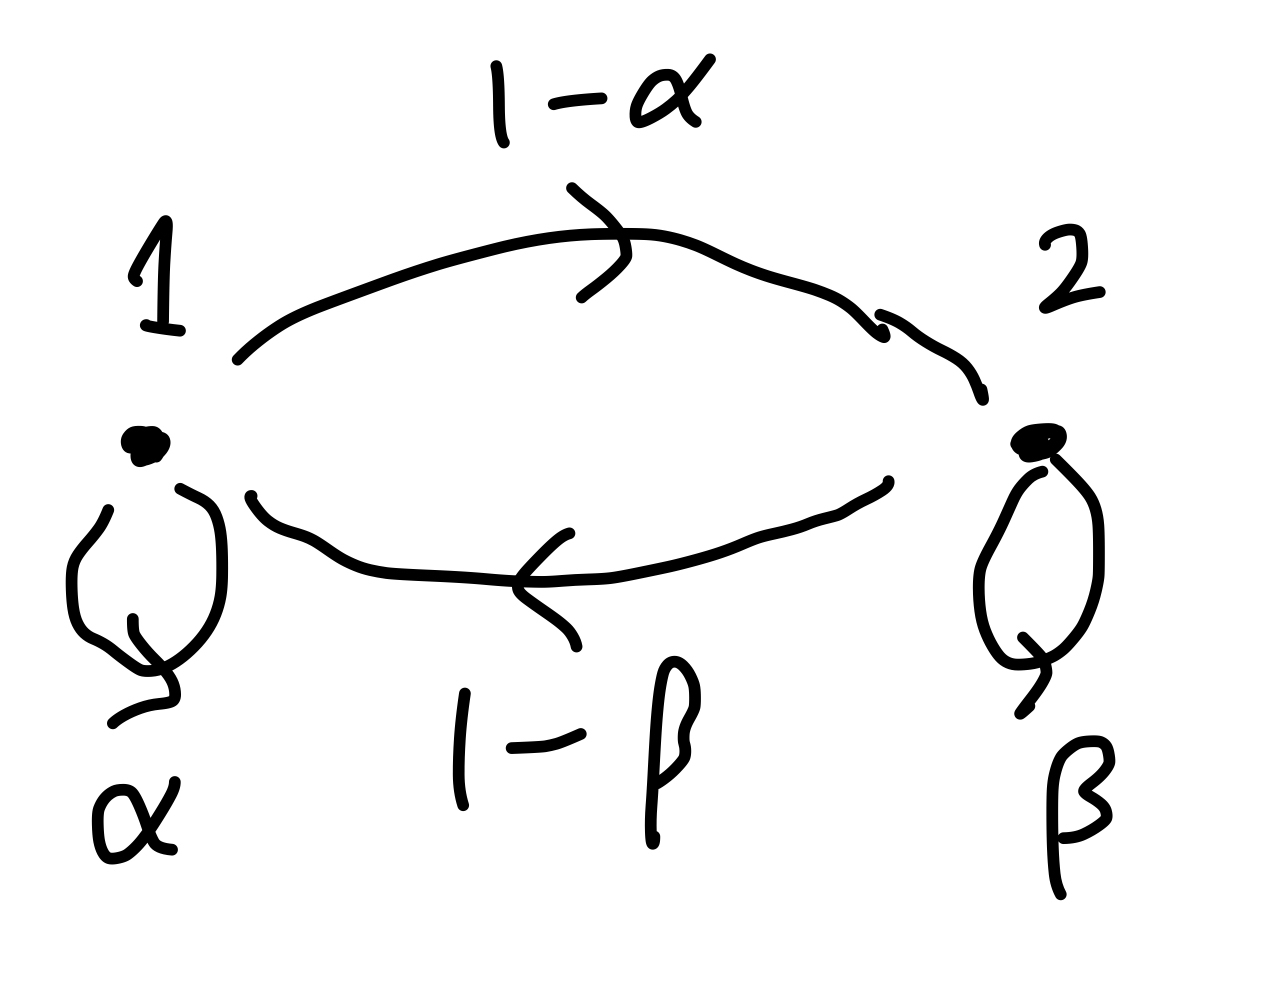
\includegraphics[scale=0.07]{markov1.jpeg}
    \end{center}
\end{example}

\begin{example}
    Let $ P = \begin{pmatrix}
        1/2 & 1/2 & 0 \\
        1/3 & 1/3 & 1/3 \\
        1 & 0 & 0 \\
    \end{pmatrix} $. The diagram is
    \begin{center}
        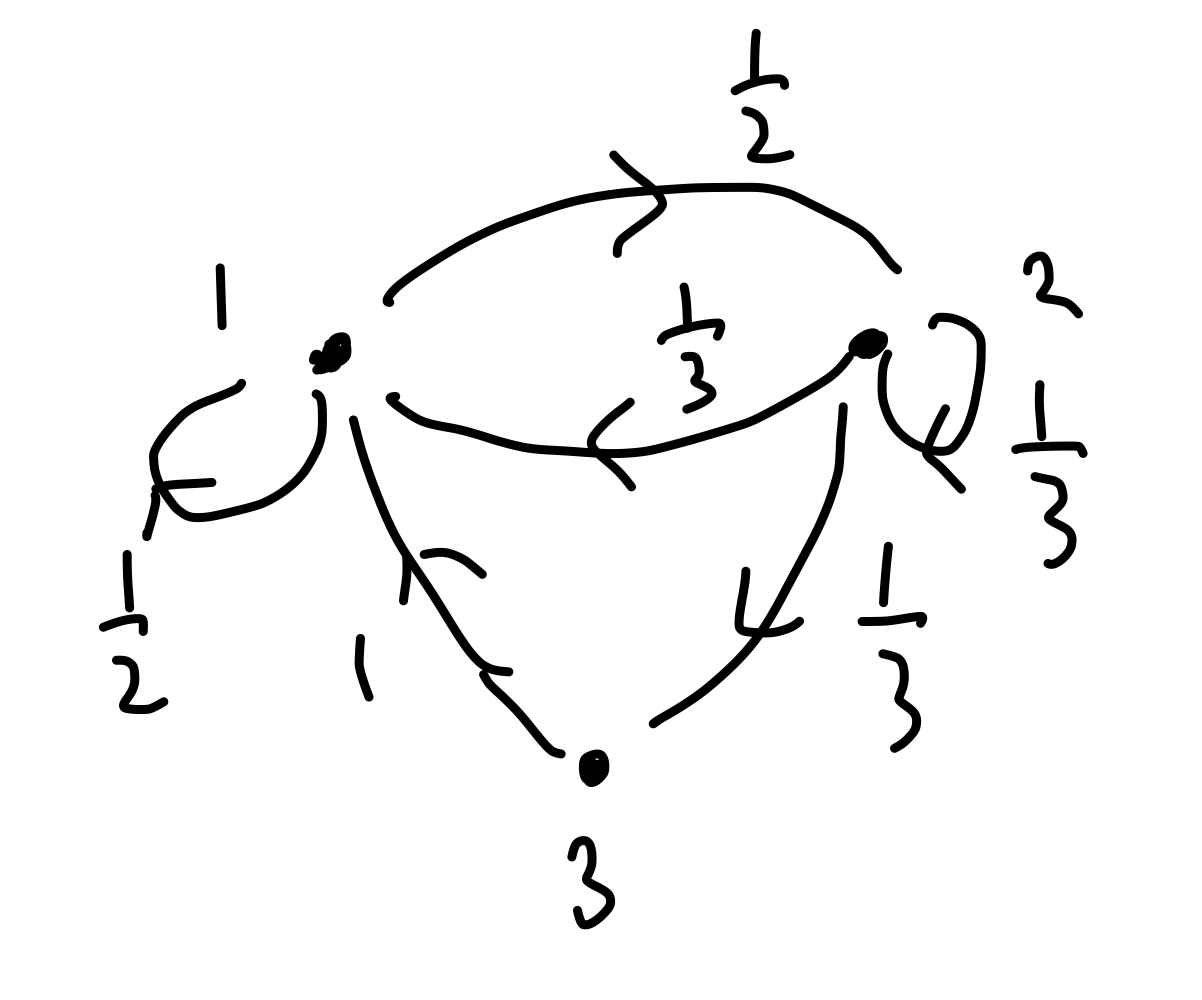
\includegraphics[scale=0.09]{markov2.jpeg}
    \end{center}
\end{example}

\section{Basic properties}

The next theorem gives the condition for $X$ to be Markov.

\begin{theorem}\label{thm:1.1}
    The process $X$ is $ \Markov(\lambda,P) $ if and only if $ \forall n\ge 0 $ and for all $ x_0,\dots,x_n\in I $, we have 
    \[
        \mathbb{P}(X_0=x_0,\dots,X_n=x_n) = \lambda_{x_0} P(x_0,x_1)\cdots P(x_{n-1},x_n).
    \]
\end{theorem}
\begin{proof}
    Suppose $ X $ is $ \Markov(\lambda,P) $. Then 
    \begin{align*}
        &\mathbb{P}(X_0=x_0,\dots,X_n=x_n)\\ &= \mathbb{P}(X_n=x_n,X_{n-1}=x_{n-1},\dots, X_0=x_0|X_{n-1}=x_{n-1},\dots, X_0=x_0)\\
        &\quad\cdot \mathbb{P}(X_{n-1}=x_{n-1},\dots, X_0=x_0 )\\
        &= \mathbb{P}(X_n=x_n|X_{n-1}=x_{n-1},\dots, X_0=x_0)\mathbb{P}(X_{n-1}=x_{n-1},\dots, X_0=x_0 )\\ 
        &= P(x_{n-1},x_n)\mathbb{P}(X_{n-1}=x_{n-1},\dots, X_0=x_0 )\\ 
        &=\cdots\\ 
        &= \mathbb{P}(X_0=x_0) P(x_0,x_1)\cdots P(x_{n-1},x_n)\\ 
        &= \lambda_{x_0} P(x_0,x_1)\cdots P(x_{n-1},x_n).
    \end{align*}

    Suppose conversely that $ \forall n\ge 0 $ and for all $ x_0,\dots,x_n\in I $, we have 
    \[
        \mathbb{P}(X_0=x_0,\dots,X_n=x_n) = \lambda_{x_0} P(x_0,x_1)\cdots P(x_{n-1},x_n).
    \]
    Setting $n=0$ gives $ \mathbb{P}(X_0=x_0)=\lambda_{x_0} $. By definition, consider 
    \begin{align*}
        &\mathbb{P}(X_n=x_n|X_{n-1}=x_{n-1},\dots, X_0=x_0)\\ &= \frac{\mathbb{P}(X_0=x_0,\dots,X_n=x_n)}{\mathbb{P}(X_0=x_0,\dots,X_{n-1}=x_{n-1})}\\ 
        &= \frac{\lambda_{x_0} P(x_0,x_1)\cdots P(x_{n-1},x_n)}{\lambda_{x_0} P(x_0,x_1)\cdots P(x_{n-2},x_{n-1})}\\ 
        &= P(x_{n-1},x_n).\qedhere
    \end{align*}
\end{proof}

\begin{definition}
    For $i\in I$ then $ \delta_i $-mass is defined as 
    \[
        \delta_{ij} = 1(i=j) = \begin{cases}
        1 &\text{if }i=j\\
        0 &\text{otherwise}\\
        \end{cases} 
    \]
\end{definition}
Recall the definition of independence: $ X_1,\dots,X_n $ are independent if $ \forall x_1,\dots,x_n\in I $, 
\[
    \mathbb{P}(X_1=x_1,\dots,X_n=x_n) = \prod_{i=1}^{n} \mathbb{P}(X_i=x_i).
\]
\begin{definition}
    A sequence $ (X_n)_{n\ge 0} $ is independent if $ \forall i_1<\cdots<i_k $ and for all $ x_1,\dots,x_k $, 
    \[
        \mathbb{P}(X_{i_1}=x_1,\dots,X_{i_k}=x_k) = \prod_{j=1}^{k}\mathbb{P}(X_{i_j}=x_j)
    \]
    Let $ X=(X_n),\ Y=(Y_n) $. $X,Y$ are independent if $ \forall k,m $ and $ \forall i_1<\cdots<i_k $, $ \forall j_1<\cdots<j_m $ we have 
    \begin{align*}
        &\mathbb{P}(X_{i_1}=x_1,\dots,X_{i_k}=x_k, Y_{j_1}=y_1,\dots,Y_{j_m}=y_m)\\
        =\;& \mathbb{P}(X_{i_1}=x_1,\dots,X_{i_k}=x_k) \mathbb{P}(Y_{j_1}=y_1,\dots,Y_{j_m}=y_m)
    \end{align*}
\end{definition}

\begin{theorem}[Simple Markov property]\label{thm:simple_markov_property}
    Suppose $ X $ is $ \Markov(\lambda,P) $ and fix $ M\in \mathbb{N}  $ and $ i\in I $. Conditional on $X_m=i$, the process $ (X_{m+n})_{n\ge 0} $ is $ \Markov(\delta_i, P) $ and it is independent of $ X_0,\dots,X_m $.
\end{theorem}
\begin{proof}
    We aim to show that $ \forall n $ and $ \forall x_i $, 
    \[
        \begin{aligned}
            &\mathbb{P}(X_{m+n}=x_{m+n},\dots,X_m=x_m|X_m=i)\\
            &= \delta_{ix_m}\mathbb{P}(X_m,X_{m+1})\cdots \mathbb{P}(X_{m+n-1},X_{m+n}).
        \end{aligned}
    \]
    We have 
    \[
        \begin{aligned}
            &\mathbb{P}(X_{m+n}=x_{m+n},\dots,X_m=x_m|X_m=i)\\ &= \frac{\mathbb{P}(X_{m+n}=x_{m+n},\dots,X_{m}=x_m)}{\mathbb{P}(X_m=i)}\delta_{ix_m}.
        \end{aligned} \tag{$ * $}
    \]
    Note that
    \begin{align*}
        &\mathbb{P}(X_{m+n}=x_{m+n},\dots,X_m=x_m)\\
        =& \sum_{x_0,\dots,x_{m-1}\in I}\mathbb{P}(X_{m+n}=x_{m+n},\dots,X_0=x_0)\tag{Result in IA Probability}\\ 
        =& \sum_{x_0,\dots,x_{m-1}\in I} \lambda x_0 \mathbb{P}(X_0,X_1)\cdots  \mathbb{P}(X_{m+n-1},X_{m+n}) \tag{Since $ X \sim \Markov(\lambda,P) $}\\ 
        =& \mathbb{P}(X_m,X_{m+1})\cdots \mathbb{P}(X_{m+n-1},X_{m+n})\mathbb{P}(X_m=x_m).
    \end{align*}
    Plugging this back into ($ * $) we get 
    \[
        \begin{aligned}
            &\mathbb{P}(X_{m+n}=x_{m+n},\dots,X_m=x_m|X_m=i)\\ &= \delta_{ix_m}\mathbb{P}(X_m,X_{m+1})\cdots \mathbb{P}(X_{m+n-1},X_{m+n}).
        \end{aligned}
    \]
    So this shows that $ (X_{m+n})_{n\ge 0} $ is $ \Markov(\delta_i,P) $ conditioning on $X_m=i$, by theorem \ref{thm:1.1}.

    To show independence, we want to show that if $ m\le i_1<\cdots<i_k,k\in \mathbb{N}  $, then 
    \begin{align*}
        &\mathbb{P}(X_{i_1}=x_{m+1},\dots,X_{i_k}=x_{m+k},X_0=x_0,\dots,X_m=x_m|X_m=i)\tag{$*$}\\ 
        =\,& \mathbb{P}(X_{i_1}=x_{m+1},\dots,X_{i_k}=x_{m+k}|X_m=i)\mathbb{P}(X_0=x_0,\dots,X_m=x_m|X_m=i).
    \end{align*}
    Note that 
    \begin{align*}
        & \mathbb{P}(X_{i_1}=x_{m+1},\dots,X_{i_k}=x_{m+k},X_0=x_0,\dots,X_m=x_m|X_m=i)\\ 
        =\,& \frac{\mathbb{P}(X_{i_1}=x_{m+1},\dots,X_{i_k}=x_{m+k},X_0=x_0,\dots,X_m=x_m)}{\mathbb{P}(X_m=i)}\tag{Assume $ x_m=i $}\\ 
        =\,& \frac{\lambda_{x_0}P(x_0,x_1)\cdots P(x_{m-1},x_m)\mathbb{P}(X_{i_1}=x_{m+1},\dots,X_{i_k}=x_{m+k}|X_m=x_m)}{\mathbb{P}(X_m=i)}\tag{Since $ X\sim \Markov(\lambda,P) $}\\ 
        =\,& \frac{\mathbb{P}(X_0=x_0,\dots,X_m=x_m)}{\bbP(X_m=i)}\mathbb{P}(X_{i_1}=x_{m+1},\dots,X_{i_k}=x_{m+k}|X_m=i)\\ 
        =\,& \mathbb{P}(X_{i_1}=x_{m+1},\dots,X_{i_k}=x_{m+k}|X_m=i)\mathbb{P}(X_0=x_0,\dots,X_m=x_m|X_m=i)
    \end{align*}
    as expected.
\end{proof}

\section{Powers of the transitional matrix}
Suppose $ X \sim \Markov(\lambda,P) $ with values in $I$. If $I$ is finite, then $ P\in \mcM_{|I|\times |I|} $ and we can label the states as $1,\dots,|I|$. If $I$ is infinite, we can label the states by $ \mathbb{N} $. Let $x\in I$ and $n\in \mathbb{N}$. Consider 
\begin{align*}
    \mathbb{P}(X_n=x)&= \sum_{x_0,\dots,x_{n-1}\in I}\mathbb{P}(X_n=x,X_{n-1}=x_{n-1},\dots,X_0=x_0)\\ 
    &= \sum_{x_0,\dots,x_{n-1}\in I} \lambda_{x_0}P(x_0,x_1)\cdots P(x_{n-1},x)\tag{By theorem \ref{thm:1.1}}
\end{align*}
We can think of $\lambda$ as a row vector and the above expression becomes $ (\lambda P^n)_x $, where $P^n$ is the $n$th power of $P$. By convention take $P^0=I$.

Let $m,n\in \bbN$. By Simple Markov Property, 
\[
    \mathbb{P}(X_{m+n}=y|X_m=x)=\mathbb{P}(X_n=y|X_0=x)=(\delta_x P^n)_y.
\]
\begin{notation}
    We will write for an event $A$: $ \mathbb{P}_i(A) $ for $ \mathbb{P}(A|X_0=i) $. We will write $ p_{ij}(n) $ for the $(i,j)$ element of $P^n$.
\end{notation}
We have proved, using these notations, that 
\begin{theorem}
    \begin{itemize}
        \item $ \mathbb{P}(X_n=x)=(\lambda P^n)_x $.
        \item $ \mathbb{P}(X_{n+m}=y|X_m=x)=\mathbb{P}_x(X_n=y)=p_{xy}(n) $.
    \end{itemize}
\end{theorem}
\begin{example}
    Take $ P = \begin{pmatrix}
        \alpha & 1-\alpha \\
        1-\beta & \beta \\
    \end{pmatrix}, \alpha,\beta\in (0,1). $
    Note that 
    \[
        p_{11}(n+1) = p_{11}(n)(1-\alpha)+p_{12}(n)\beta.
    \]
    Since $P$ is a stochastic matrix, $P_{11}(n)+P_{12}(n)=1 $, and thus 
    \[
        p_{11}(n+1)=(1-\alpha-\beta)P_{11}(n)+\beta.
    \]
    We can now solve this recursion to get 
    \[
        p_{11}(n)=\begin{cases}
        \frac{\alpha}{\alpha+\beta}\left( 1+(1-\alpha-\beta)^n \right) &\text{if }\alpha+\beta>0\\
        1 &\text{if }\alpha+\beta=0\\
        \end{cases} 
    \]
\end{example}
\paragraph*{General procedure for $ P^n $} Suppose $P$ is a $k\times k$ matrix and let $ \lambda_1,\dots,\lambda_k $ be its eigenvalues.
\begin{enumerate}[(1)]
    \item \textit{All $ \lambda_i $ are distinct.} Then $P$ is diagonalisable and we can write 
    \[
        P = U \begin{pmatrix}
            \lambda_1&&&0\\ 
            &\lambda_2&&\\ 
            &&\ddots&\\ 
            0&&&\lambda_k
        \end{pmatrix}U^{-1} \Longrightarrow P^n=U \begin{pmatrix}
            \lambda^n_1&&&0\\ 
            &\lambda^n_2&&\\ 
            &&\ddots&\\ 
            0&&&\lambda^n_k
        \end{pmatrix}U^{-1}
    \]
    Suppose, for example, that we want to find $p_{11}(n)$. We can write 
    \[
        p_{11}(n)=a_1 \lambda_1^n+\cdots + a_k \lambda_k^n,\quad a_1,\dots,a_k \text{ are constants}.
    \]
    We can then determine $a_i$ by plugging in small values of $n$ and solve the linear equations.

    Suppose $\lambda_k$ is complex. Also $ \bar{\lambda}_k $ will be an eigenvalue. Write $ \lambda_k=re^{i\theta}, \bar{\lambda}_k=\lambda_{k-1}=re^{-i\theta} $. Since $p_{11}(n)$ is always real, we can write directly
    \[
        p_{11}(n)=a_1 \lambda_1^n+\cdots + a_{k-2}\lambda_{k-2}^n+a_{k-1}r^{n}\cos (n\theta)+a_kr^n \sin (n\theta).
    \]
    \item \textit{If they are not all distinct}, then say $ \lambda $ appears with multiplicity 2, then we include also the term $ (an+b)\lambda^n $ instead of just $ b\lambda^n $. (Jordan normal form of $P$)
\end{enumerate}

\begin{example}
	Given the transition matrix
	$$
	P = \begin{pmatrix}
		0 & 1 & 0 \\
		0 & 1/2 & 1/2 \\ 
		1/2 & 0 & 1/2
	\end{pmatrix},
	$$
	we want to find $p_{11}(n)$. The eigenvalues are $1, \pm i/2$. We write $\pm i/2 = (\cos \pi/2 \pm i \sin \pi/2)/2$, and thus the general form of $p_{11}(n)$ as
	$$
	p_{11}(n) = \alpha + \beta \cdot \left(\frac{1}{2}\right)^n \cos \left(\frac{n \pi}{2}\right) + \gamma \cdot \left(\frac{1}{2}\right)^n \sin\left(\frac{n \pi}{2}\right).
	$$
	Plug in $p_{11}(0) = 1$, $p_{11}(1) = 0$ and $p_{11}(2) = 0$ to get
	$$
	p_{11}(n) = \frac{1}{5} + \left(\frac{1}{2}\right)^n \left(\frac{4}{5}\cos\left(\frac{n \pi}{2}\right) - \frac{2}{5} \sin \left(\frac{n \pi}{2}\right)\right).
	$$
\end{example}

\section{Communicating classes}
\begin{definition}
    Let $X$ be a Markov chain with transition matrix $P$ and values in $I$. For $x, y \in I$ we say that \textbf{$x$ leads to $y$} and write it $x \rightarrow y$ if
    $$
    \mathbb{P}(X_n = y \text{ for some }n \ge 0) > 0. 
    $$
    We say that $x$ \textbf{communicates} with $y$ and write $x \leftrightarrow y$ if $x \rightarrow y$ and $y \rightarrow x$.  
\end{definition}

\begin{theorem}
	The following are equivalent: 
	\begin{enumerate}[label=(\roman*)]
		\item $x \rightarrow y$;
		\item There exists a sequence of states $x = x_0, x_1, \dots, x_k = y$ such that 
		$$P(x_0, x_1)P(x_1, x_2) \cdots P(x_{k - 1}, x_k) > 0;$$
		\item There exists $n \ge 0$ such that $p_{xy}(n) > 0$.
	\end{enumerate}
\end{theorem}
\begin{proof}
    ((i) $ \Leftrightarrow $ (iii)) Note that 
    \[
        \{X_n=y \text{ for some }n\ge 0\} = \bigcup_{n=0}^{\infty}\{X_n=y\}.
    \]
    If $ \mathbb{P}(X_n = y \text{ for some }n \ge 0) > 0 $, then $ \exists n\ge 0 $ such that $ \mathbb{P}_x(X_m=y)=p_{xy}(n)>0 $.

    If $ \exists n\ge 0 $ such that $ p_{xy}(n)>0 $, then 
    \[
        \{X_n=y \text{ for some }n\ge 0\}=\mathbb{P}\left( \bigcup_{n=0}^{\infty}\{X_n=y\} \right)>0.
    \]

    ((ii) $ \Leftrightarrow  $ (iii)) Note that $ p_{xy}(n) = \sum_{x_0,\dots x_{n-1}} P(x,x_1)P(x_1,x_2)\cdots P(x_{n-1},y), $
    so they are equivalent.
\end{proof}
\begin{corollary}
    $ \leftrightarrow $ is an equivalence relation on $I$.
\end{corollary}
\begin{definition}[Communicating Classes]
	The equivalence classes induced by $\leftrightarrow$ on $I$ are called \textbf{communicating classes}.

    A communicating class $C$ is \textbf{closed} if $x \in C$ and $x \rightarrow y$ then $y \in C$.

    A matrix $P$ is called \textbf{irreducible} if it has a single communicating class, that is, for all $x, y \in I$, $x \leftrightarrow y$. 

    A state $x$ is called \textbf{absorbing} if $\{x\}$ is a closed class. 
\end{definition}

\section{Hitting Times}

\begin{definition}
	We define $T_A$ to be the first hitting time of $A$, i.e. $T_A$ is a random variable $T_A: \Omega \rightarrow\{0,1, \ldots\} \cup\{\infty\}$ given by
    \[
    T_A(\omega)=\inf \left\{n \geq 0: X_n(\omega) \in A\right\} .
    \]
    We use the convention that the infimum of the empty set is equal to $\infty$.

    The \textbf{hitting probability} of $A$ is defined to be the function $h^A: I \rightarrow[0,1]$ given by
    \[
    h_i^A=\mathbb{P}_i\left(T_A<\infty\right) .
    \]
    The \textbf{mean hitting time} of $A$ is defined to be the function $k^A: I \rightarrow \mathbb{R}_{+} \cup\{\infty\}$ given by
    \[
    k_i^A=\mathbb{E}_i\left[T_A\right]=\sum_{n=0}^{\infty} n \mathbb{P}_i\left(T_A=n\right)+\infty \cdot \mathbb{P}_i\left(T_A=\infty\right)
    \]
\end{definition}

\begin{example}
	Consider the Markov chain in the diagram below.
	\begin{center}
		\begin{tikzpicture}
		
		\node[state] (1) {1};
		\node[state, right=of 1] (2) {2};
		\node[state, right=of 2] (3) {3};
		\node[state, right=of 3] (4) {4};
		
		\path
		(2) edge[->,above] node {$\frac{1}{2}$} (1)
		(2) edge[bend left, ->,above] node {$\frac{1}{2}$} (3)
		(3) edge[bend left, ->,below] node {$\frac{1}{2}$} (2)
		(3) edge[->,above] node {$\frac{1}{2}$} (4);
		\end{tikzpicture}
		\end{center}

		We take $A = \{4\}$, and want to find $h_2^A = \bbP_2(T_A < \infty)$. We have
		\begin{align*}
			h_2^A &= \frac{1}{2}h_1^A +
			\frac{1}{2}h_3^A =\frac{1}{2}\left( \frac{1}{2}+\frac{1}{2}h_2^A \right) \\
		\implies h_2^A &= \frac{1}{3}.
		\end{align*}
		If instead we took $B = \{1, 4\}$ and wanted to find $k_2^B$, we would get
		\begin{align*}
			k_2^B &= 1+\frac{1}{2}k_1^B+\frac{1}{2}k_3^B=\frac{1}{2}\left( 1+\frac{1}{2}k_4^B+\frac{1}{2}k_2^B \right)=\frac{1}{2}\left( 1+\frac{1}{2}k_2^B \right)\\
	\implies k_2^B &= 2.
		\end{align*}
\end{example}
\subsection{Absorption probabilities are minimal solutions}
\begin{theorem}
	Let $A \subseteq I$. The vector $(h_i^A)_{i \in I}$ is the minimal non-negative solution to
	\begin{align*}
		h_i^A = \begin{cases}
			1 &\mbox{if } i  \in A, \\
			\sum_{j} P(i, j) h_j^A &\mbox{if } i \not \in A,
		   \end{cases}
	\end{align*}
	where minimality means that if $(x_i)_{i \in A}$ is another solution to the linear system, then $x_i \ge h_i^A, \forall i$.
\end{theorem}
\begin{proof}
	First show that $(h_i)$ solves this system. Clearly, if $i\in A$ then $ h_i^A=1 $. Suppose $i\notin A$. Note that 
    \[
        \{T_A<\infty\} = \{X_0\in A\} \cup \bigcup_{n=1}^{\infty}\{X_i\notin A \text{ for }0\le i\le n-1, X_n\in A\}.
    \]
    By countable additivity of disjoint events,
    \begin{align*}
        &\mathbb{P}_i(T_A< \infty)={\color{blue}h_i^A} =\sum_{n=1}^{\infty}\mathbb{P}(X_0\notin A,\dots,X_{n-1}\notin A, X_n\in A|X_0=i)\\ 
            &= \sum_{n=1}^{\infty} \sum_{j} \mathbb{P}(X_0\notin A,\dots,X_{n-1}\notin A, X_n\in A|X_0=i,X_1=j)P(i,j)\\ 
            &=\sum_j \mathbb{P}(\cancel{X_0\notin A}, X_1\in A|\cancel{X_0=i},X_1=j)P(i,j)\\[-1em]
            &\hspace{4em}+\sum_j \sum_{n=2}^{\infty}\mathbb{P}(X_0\notin A,\dots,X_{n-1}\notin A, X_n\in A|X_0=i,X_1=j)P(i,j)\\ 
            &=\sum_j P(i,j)\mathbb{P}(X_1\in A|X_1=j)\\[-1em]
            &\hspace{4em}+\sum_j \sum_{n=1}^{\infty}P(i,j)\mathbb{P}(X_0\notin A,\dots,X_{n-1}\notin A, X_n\in A|X_1=j)\tag{By Simple Markov Property} \\
            &= \sum_j P(i,j) \left( \mathbb{P}_j(X_0\in A)+\sum_{n=1}^{\infty} \mathbb{P}_j(X_0\notin A,\dots,X_{n-1}\notin A, X_n\in A)\right)\tag{Combine terms and add `zero' term $\mathbb{P}_j(X_0\in A)$}\\ 
            &= \sum_j P(i,j) \left( \mathbb{P}_j(T_A=0)+ \sum_{n=1}^{\infty}\mathbb{P}_j(T_A=n) \right)\\ 
            &= \sum_j P(i,j) \bbP_j(T_A< \infty ) = {\color{blue}\sum_j P(i,j)h_j^A}.
    \end{align*}
    Hence it is a solution.

    We now check minimality. Let $x = (x_i \mid i \in S)$ be another non-negative solution. For $i \in A$, we have $x_i = h^A_i = 1$, so that holds. Then for $i \in S \backslash A$, since $x$ satisfies the system of equations we can write
	\begin{equation}\label{eq:1}
		x_i = \sum_{j \in S}P_{i, j} x_j = \sum_{j \in A} P_{i, j} x_j + \sum_{j \in S \backslash A} P_{i, j} x_j. \tag{$\dagger$}
	\end{equation}
	Then with $x_j = 1$ for $j \in A$ and $x \geq 0$, we have
	\begin{align*}
		x_i \geq \sum_{j \in A} P_{i, j} = \bbP(X_1 \in A \mid X_0 = i) = \bbP(T_A < 2 \mid X_0 = i).
	\end{align*}
	Similarily, expanding \eqref{eq:1}, we have
	\begin{align*}
	x_i &= \bbP(X_1 \in A \mid X_0 = i) + \sum_{j \in S \backslash A} P_{i, j} \left(\sum_{k \in A} P_{j, k} x_k + \sum_{k \in S \backslash A} P_{j, k} x_k\right) \\
		&\geq \bbP(X_1 \in A \mid X_0 = i) + \bbP(X_1 \not \in A, X_2 \in A \mid X_0 = i) \\
		&= \bbP(T_A < 3 \mid X_0 = 1).
	\end{align*}
	We can repeat this argument to eventually establish that $x_i \geq \bbP(T_A < n \mid X_0 = i)$, for all $n \geq 0$. Then as $n \rightarrow \infty$, we have $x_i \geq \bbP(T_A < \infty \mid X_0 = i)$, as required.
\end{proof}

This method of computing hitting probabilities is perfectly valid on Markov chains with infinite state spaces.

\begin{example}
    Consider again the Markov chain in the diagram below.
	\begin{center}
		\begin{tikzpicture}
		
		\node[state] (1) {1};
		\node[state, right=of 1] (2) {2};
		\node[state, right=of 2] (3) {3};
		\node[state, right=of 3] (4) {4};
		
		\path
		(2) edge[->,above] node {$\frac{1}{2}$} (1)
		(2) edge[bend left, ->,above] node {$\frac{1}{2}$} (3)
		(3) edge[bend left, ->,below] node {$\frac{1}{2}$} (2)
		(3) edge[->,above] node {$\frac{1}{2}$} (4);
		\end{tikzpicture}
		\end{center}
    Take $A=\{4\}$. Applying the theorem, 
    \begin{align*}
        h_2&= \frac{1}{2}h_1+\frac{1}{2}h_3\\ 
        h_3&= \frac{1}{2}h_4+\frac{1}{2}h_2\\ 
        h_4&=1
    \end{align*}
    Then we can solve as before.
\end{example}
\begin{example}
	Consider the Markov chain with states $S = \{0, 1, \dots\}$ such that $P_{0, 1} = 1$, and
	$$
	P_{i, i+1} = p, \quad P_{i, i - 1} = q \quad \text{for all } i \geq 1,
	$$ 
	where $p, q \in (0, 1)$ with $p + q = 1$.

	\begin{center}
    \begin{tikzpicture}
    
    \node[state] (1) {1};
    \node[state, right=of 1] (2) {2};
    \node[state, right=of 2] (3) {3};
    \node[state, right=of 3] (4) {4};
    \node[state, right=of 4] (5) {$\cdots$};
    
    \path
    (1) edge[above,->] node {1} (2)
    (2) edge[above,->] node {$p$} (3)
    (3) edge[above,->] node {$p$} (4)
    (4) edge[above,->] node {$\cdots$} (5)
    (2) edge[bend left, below,->] node {$q$} (1)
    (3) edge[bend left, below,->] node {$q$} (2)
    (4) edge[bend left, below,->] node {$q$} (3)
    (5) edge[bend left, below,->] node {$\cdots$} (4);
    \end{tikzpicture}
    \end{center}

	Let $h_i = \bbP(T_0 < \infty \mid X_0 = i)$, and suppose that $p \neq q$. $h_0 = 1$, and generally
	$$
		h_i = p h_{i + 1} + qh_{i - 1}.
	$$
	This then implies $p(h_{i + 1} - h_i) = q(h_{i} - h_{i - 1})$, so that
	$$
		h_{i+1} - h_{i}  = \left(\frac{q}{p}\right)^i (h_1 - 1).
	$$
	This inspires us to write $h_i$ as a telescoping sum
	\begin{align*}
		h_i &= \sum_{j = 1}^i (h_j - h_{j - 1}) + 1  \\
			&= (h_1 - 1) \sum_{j = 1}^i \left(\frac{q}{p}\right)^j + 1,
	\end{align*}
	which gives us our general solution $h_i = a + b(q/p)^i$, which we can then solve.

	If $q > p$, then in order for $h_i$ to be the minimal solution, we need to have $a = 1$ and $b = 0$, so $h_i = 1$.

    If $p>q$ then in seeking a minimal solution we will wish to take $A$ as large as possible, consistent with $h_{i} \geq 0$ for all $i$. So $a=0,b=1$, and $h_{i}=(q / p)^{i}$.

    Finally, if $p=q=1 / 2$ the recurrence relation has a general solution $h_{i}=a+b i$, and the restriction $0 \leq h_{i} \leq 1$ forces $a=1,b=0$. Thus $h_{i}=1$ for all $i$. So even if you find a fair casino you are certain to end up broke. This apparent paradox is called \textit{gambler's ruin}.
\end{example}

\begin{example}[Birth and Death Chains]
	Consider the Markov chain with diagram
    \begin{center}
        \begin{tikzpicture}
        
        \node[state] (1) {0};
        \node[state, right=of 1] (2) {1};
        \node[state, right=of 2] (3) {$i-1$};
        \node[state, right=of 3] (4) {$i$};
        \node[state, right=of 4] (5) {$i+1$};
        \node[state, right=of 5] (6) {$\cdots$};
        
        \path
        (1) edge[above,->] node {1} (2)
        (2) edge[above,->] node {$\cdots$} (3)
        (3) edge[above,->] node {$p_{i-1}$} (4)
        (4) edge[above,->] node {$p_i$} (5)
        (2) edge[bend left, below,->] node {$q_1$} (1)
        (3) edge[bend left, below,->] node {$\cdots$} (2)
        (4) edge[bend left, below,->] node {$q_i$} (3)
        (5) edge[bend left, below,->] node {$q_{i+1}$} (4)
        (5) edge[above,->] node {$\cdots$} (6)
        (6) edge[bend left, below,->] node {$\cdots$} (5);
        \end{tikzpicture}
        \end{center}
        where, for $i=1,2, \ldots$, we have $0<p_{i}=1-q_{i}<1$. State $i$ is that in which a population is $i$.

    As in previous examples, 0 is an absorbing state and we wish to calculate the absorption probability starting from state $i$. So now $h_{i}=\mathbb{P}_i(\text{hit 0})$ is the extinction probability starting from state $i$. We write down the usual system of r.h. equations
    \[
    \begin{aligned}
    h_{0} &=1 \\
    h_{i} &=p_{i} h_{i+1}+q_{i} h_{i-1} \quad \text { for } i=1,2, \ldots
    \end{aligned}
    \]
    This recurrence relation has variable coefficients so the usual technique fails. But consider $u_{i}=h_{i-1}-h_{i} .$ Then $p_{i} u_{i+1}=q_{i} u_{i}$, so
    \[
    u_{i+1}=\left(\frac{q_{i}}{p_{i}}\right) u_{i}=\left(\frac{q_{i} q_{i-1} \cdots q_{1}}{p_{i} p_{i-1} \cdots p_{1}}\right) u_{1}=\gamma_{i} u_{1}
    \]
    where the final equality defines $\gamma_{i} $. Then
    \[
    u_{1}+\cdots+u_{i}=h_{0}-h_{i}
    \]
    So
    \[
    h_{i}=1-u_{1}\left(\gamma_{0}+\cdots+\gamma_{i-1}\right)
    \]
    where $\gamma_{0}=1$. At this point $u_{1}$ remains to be determined. Since we know $h$ is the minimal solution to the right hand equations, we want to choose $u_{1}$ to be as large as possible. In the case $\sum_{i=0}^{\infty} \gamma_{i}=\infty$, the restriction $0 \leq h_{i} \leq 1$ forces $u_{1}=1-h_{1}=0$ and $h_{i}=1$ for all $i .$ But if $\sum_{i=0}^{\infty} \gamma_{i}<\infty$ then we can take $u_{1}>0$ so long as
    \[
    1-u_{1}\left(\gamma_{0}+\cdots+\gamma_{i-1}\right) \geq 0 \quad \text { for all } i
    \]
    Thus the minimal non-negative solution occurs when $u_{1}=\left(\sum_{i=0}^{\infty} \gamma_{i}\right)^{-1}$ and then
    \[
    h_{i}=\sum_{j=i}^{\infty} \gamma_{j}\bigg/\sum_{j=0}^{\infty} \gamma_{j}
    \]
    In this case, for $i=1,2, \ldots$, we have $h_{i}<1$, so the population survives with positive probability. 
\end{example}
\subsection{Mean hitting times are minimal solutions}
\begin{theorem}
    The vector of mean hitting times $k^{A}=\left(k_{i}^{A}: i \in I\right)$ is the minimal non-negative solution to the system of linear equations
    \[
    \begin{cases}k_{i}^{A}=0 & \text { for } i \in A \\ k_{i}^{A}=1+\sum_{j} p_{i j} k_{j}^{A} & \text { for } i \notin A\end{cases}
    \]
\end{theorem}
\begin{proof}
    First we show that $k^{A}$ satisfies the equation. If $X_{0}=i \in A$, then $T^{A}=0$, so $k_{i}^{A}=0$. If $X_{0} \notin A$, then $T^{A} \geq 1$, so by the Markov property
    \[
    \bbE_{i}\left(T^{A} \mid X_{1}=j\right)=1+\bbE_{j}\left(T^{A}\right)=1+k_{j}^{A}
    \]
    and so for $i \notin A$,
    \[
    \begin{aligned}
    k_{i}^{A} &=\sum_{t=1}^{\infty} \bbP\left(T^{A} \geq t\right)=\sum_{t=1}^{\infty} \sum_{j \in I} \bbP\left(T^{A} \geq t \mid X_{1}=j\right) \bbP_{i}\left(X_{1}=j\right) \\
    &=\sum_{j \in I} \sum_{t=1}^{\infty} \bbP\left(T^{A} \geq t \mid X_{1}=j\right) \bbP_{i}\left(X_{1}=j\right) \\
    &=\sum_{j \in I} \bbE_{i}\left(T^{A} \mid X_{1}=j\right) \bbP_{i}\left(X_{1}=j\right) \\
    &=\sum_{j \in I} p_{i j}\left(1+k_{j}^{A}\right) \\
    &=1+\sum_{j \in I} p_{i j} k_{j}^{A}
    \end{aligned}
    \]
    In the second line above we use the fact that we can swap $\sum_{t \geq 1}$ and $\sum_{j \in I}$ for countable sums (Fubini's theorem).

    Suppose now that $y=\left(y_{i}: i \in I\right)$ is any solution to (4.1). Then $k_{i}^{A}=y_{i}=0$ for $i \in A$. Suppose $i \notin A$, then
    \[
    \begin{aligned}
    y_{i} &=1+\sum_{j \notin A} p_{i j} y_{j} \\
    &=1+\sum_{j \notin A} p_{i j}\left(1+\sum_{k \notin A} p_{j k} y_{k}\right) \\
    &=\bbP_{i}\left(T^{A} \geq 1\right)+\bbP_{i}\left(T^{A} \geq 2\right)+\sum_{j, k \notin A} p_{i j} p_{j k} y_{k}
    \end{aligned}
    \]
    By repeated substitution we obtain
    \[
    y_{i}=\bbP_{i}\left(T^{A} \geq 1\right)+\cdots+\bbP_{i}\left(T^{A} \geq n\right)+\sum_{j_{1}, \ldots, j_{n} \notin A} p_{i j_{1}} p_{j_{1} j_{2}} \cdots p_{j_{n-1} j_{n}} y_{j_{n}}
    \]

    So since $y_{j_{n}}$ is non-negative
    \[
    y_{i} \geq \lim _{n \rightarrow \infty}\left[\bbP_{i}\left(H^{A} \geq 1\right)+\cdots+\bbP_{i}\left(T^{A} \geq n\right)\right]=\bbE_{i}\left(T^{A}\right)=k_{i}^{A}.
    \]
\end{proof}

\section{Strong Markov property}
\end{document}